% ==============================================================================
%
%                                    DVG303
%                  Objektorienterad design och programmering
%                                Laboration #1
%
% Author:   Jonas Sjöberg
%           Högskolan i Gävle
%           tel12jsg@student.hig.se
%           https://github.com/jonasjberg
%
% License:  Creative Commons Attribution-NonCommercial-ShareAlike 4.0
%           International.  See LICENSE.md for full licensing information.
% ==============================================================================

\section{Introduktion}\label{sec:intro}

\subsection{}\label{sec:uppg1a}
\subsubsection*{Övergripande beskrivning}
Det här är den första av tre laborationer i objektorienterad design och
programmering. Under laborationerna kommer programvara att utvecklas från en
specifikation. 
% TODO: Syfte (modern mjukvaruutveckling, revisionskontroll, dokumentation ..)

\subsubsection*{Specifikation}
Efterfrågad funktionalitet för programmet beskrivs enligt UML-standard i 
Figur~\ref{fig:usecase}.

\begin{figure}[htbp]
\centering
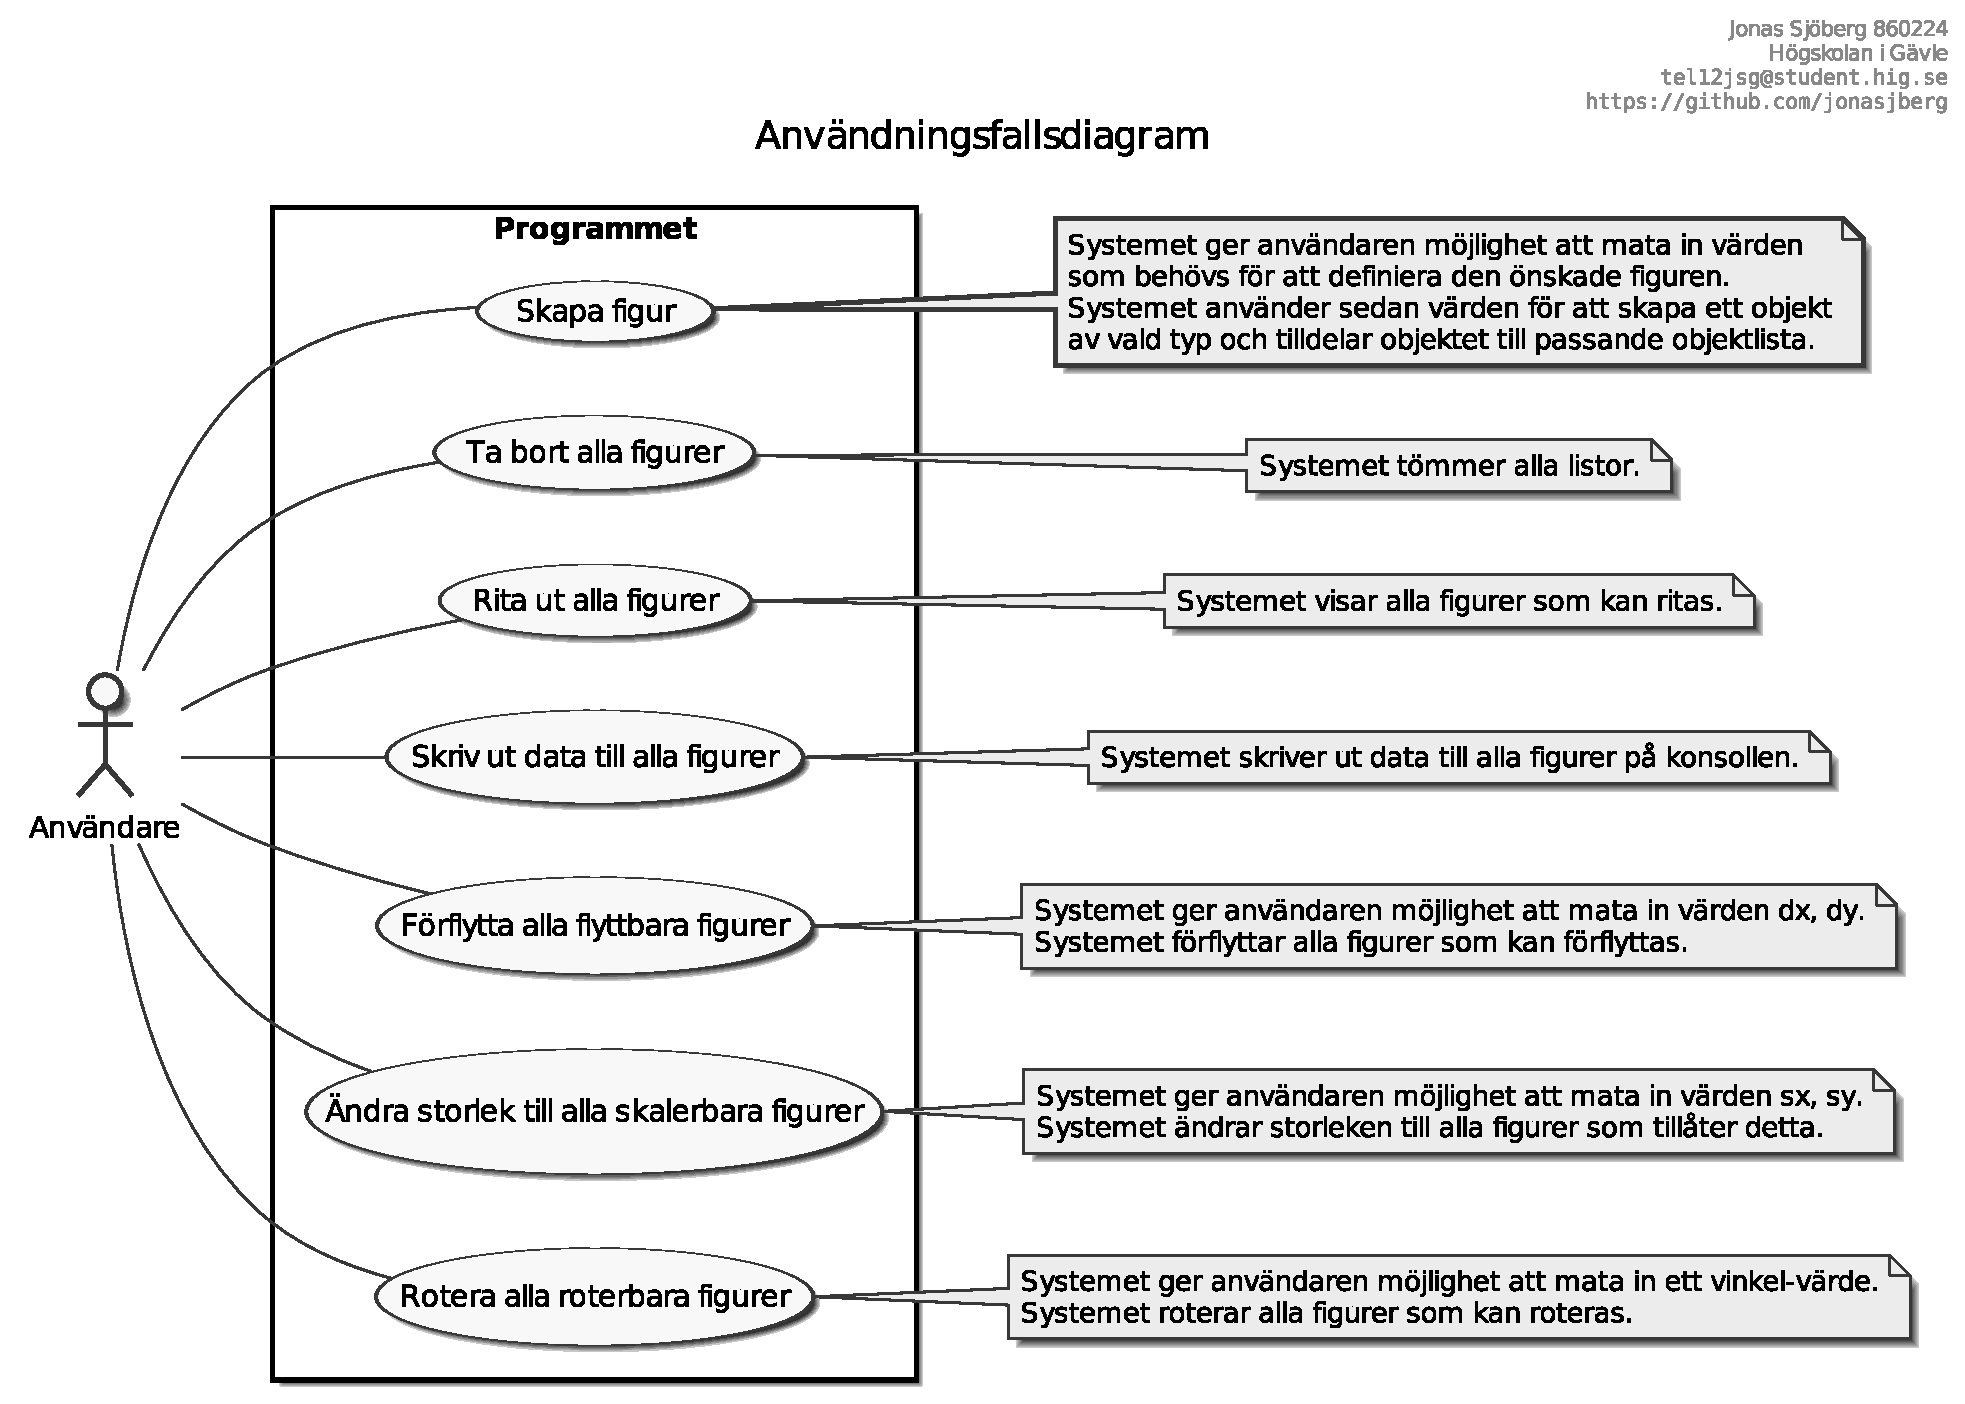
\includegraphics[width=\linewidth]{diagram/usecase.eps}
\caption{Användningsfallsdiagram \emph{("use case diagram")}}
\label{fig:usecase}
\end{figure}



